\documentclass[11pt,a4paper]{report}
\usepackage[textwidth=37em,vmargin=30mm]{geometry}
\usepackage{calc,xunicode,amsmath,amssymb,paralist,enumitem,tabu,booktabs,datetime2,xeCJK,xeCJKfntef,listings}
\usepackage{tocloft,fancyhdr,tcolorbox,xcolor,graphicx,eso-pic,xltxtra,xelatexemoji}

\newcommand{\envyear}[0]{2025}
\newcommand{\envdatestr}[0]{2025-01-18}
\newcommand{\envfinaldir}[0]{webdb/2025/20250118/final}

\usepackage[hidelinks]{hyperref}
\hypersetup{
    colorlinks=false,
    pdfpagemode=FullScreen,
    pdftitle={Web Digest - \envdatestr}
}

\setlength{\cftbeforechapskip}{10pt}
\renewcommand{\cftchapfont}{\rmfamily\bfseries\large\raggedright}
\setlength{\cftbeforesecskip}{2pt}
\renewcommand{\cftsecfont}{\sffamily\small\raggedright}

\setdefaultleftmargin{2em}{2em}{1em}{1em}{1em}{1em}

\usepackage{xeCJK,xeCJKfntef}
\xeCJKsetup{PunctStyle=plain,RubberPunctSkip=false,CJKglue=\strut\hskip 0pt plus 0.1em minus 0.05em,CJKecglue=\strut\hskip 0.22em plus 0.2em}
\XeTeXlinebreaklocale "zh"
\XeTeXlinebreakskip = 0pt


\setmainfont{Brygada 1918}
\setromanfont{Brygada 1918}
\setsansfont{IBM Plex Sans}
\setmonofont{JetBrains Mono NL}
\setCJKmainfont{Noto Serif CJK SC}
\setCJKromanfont{Noto Serif CJK SC}
\setCJKsansfont{Noto Sans CJK SC}
\setCJKmonofont{Noto Sans CJK SC}

\setlength{\parindent}{0pt}
\setlength{\parskip}{8pt}
\linespread{1.15}

\lstset{
	basicstyle=\ttfamily\footnotesize,
	numbersep=5pt,
	backgroundcolor=\color{black!5},
	showspaces=false,
	showstringspaces=false,
	showtabs=false,
	tabsize=2,
	captionpos=b,
	breaklines=true,
	breakatwhitespace=true,
	breakautoindent=true,
	linewidth=\textwidth
}






\newcommand{\coverpic}[2]{
    % argv: itemurl, authorname
    Cover photo by #2~~(\href{#1}{#1})
}
\newcommand{\makeheader}[0]{
    \begin{titlepage}
        % \newgeometry{hmargin=15mm,tmargin=21mm,bmargin=12mm}
        \begin{center}
            
            \rmfamily\scshape
            \fontspec{BaskervilleF}
            \fontspec{Old Standard}
            \fontsize{59pt}{70pt}\selectfont
            WEB\hfill DIGEST
            
            \vfill
            % \vskip 30pt
            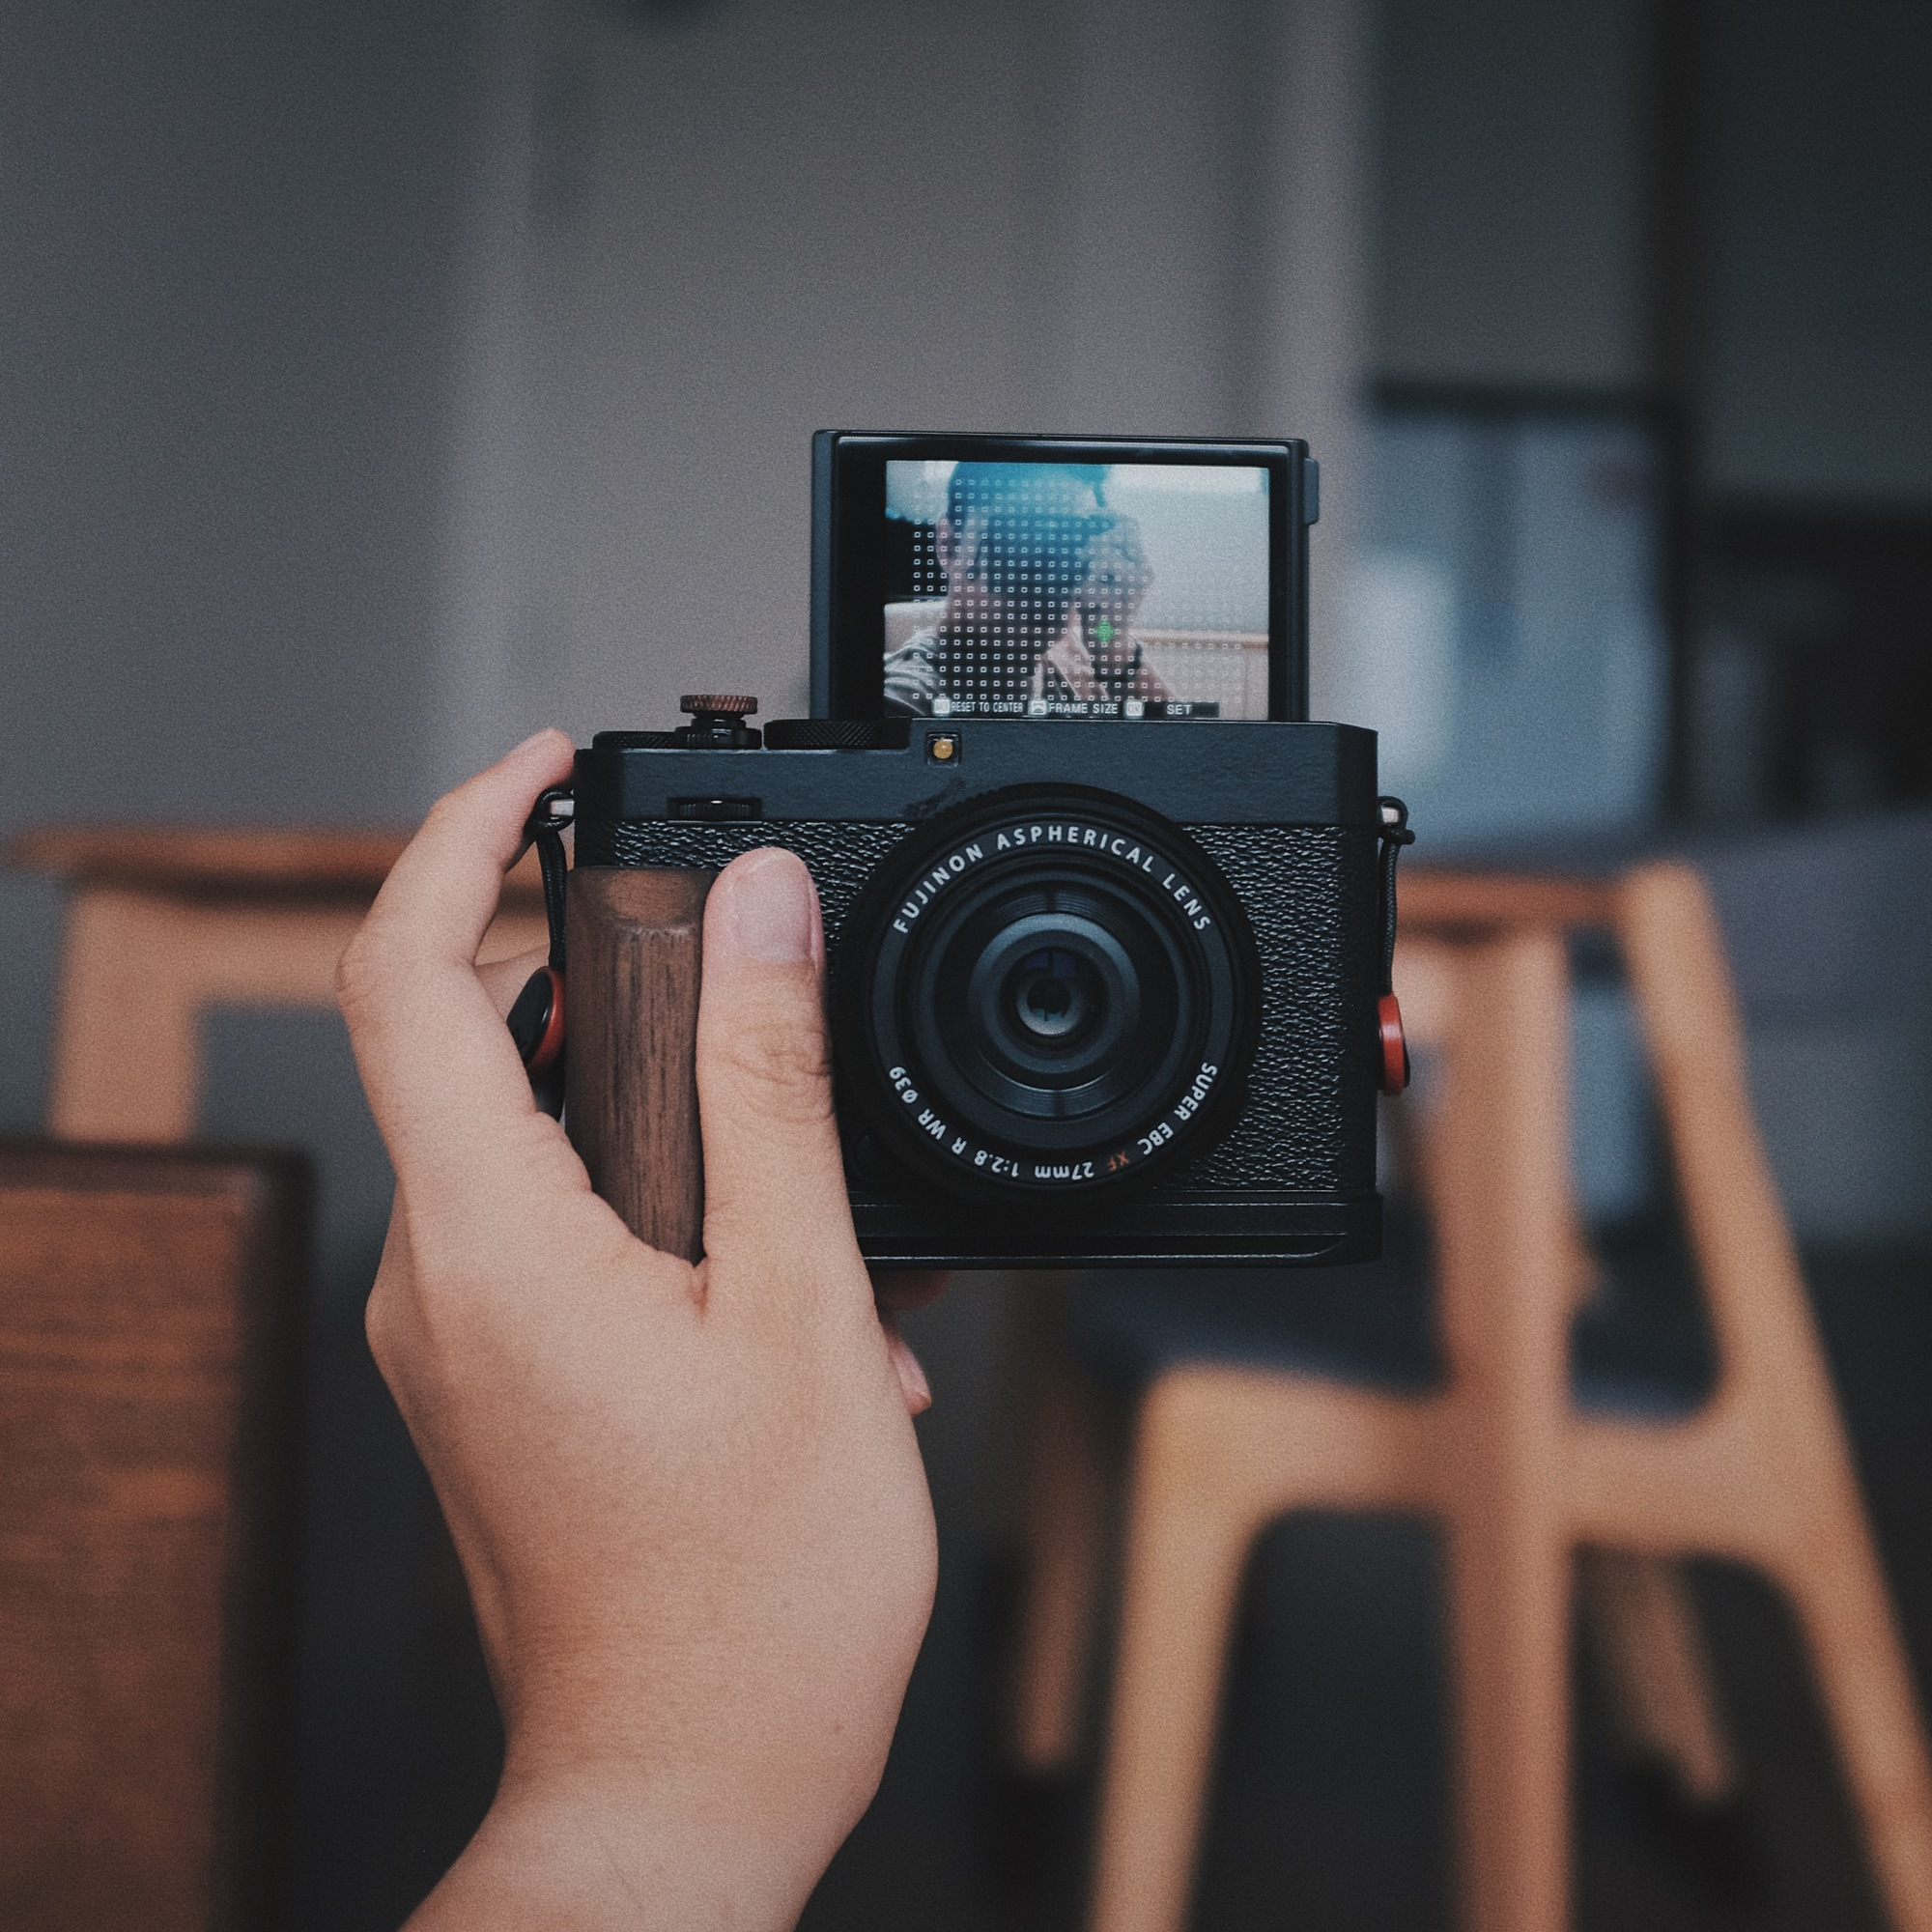
\includegraphics[width=\linewidth]{\envfinaldir/coverpic-prod.jpg}\par
            % \vskip 30pt
            \vfill

            \normalsize\rmfamily\scshape
            \copyright{} The Web Digest Project \hfill\large \envdatestr
        \end{center}
    \end{titlepage}
    % \restoregeometry
}
\newcommand{\simplehref}[1]{%
    \textcolor{blue!80!green}{\href{#1}{#1}}%
}
\renewcommand{\contentsname}{\center\Huge\sffamily\bfseries Contents\par\vskip 20pt}
\newcounter{ipartcounter}
\setcounter{ipartcounter}{0}
\newcommand{\ipart}[1]{
    % \vskip 20pt
    \clearpage
    \stepcounter{ipartcounter}
    \phantomsection
    \addcontentsline{toc}{chapter}{#1}
    % \begin{center}
    %     \Huge
    %     \sffamily\bfseries
    %     #1
    % \end{center}
    % \vskip 20pt plus 7pt
}
\newcounter{ichaptercounter}
\setcounter{ichaptercounter}{0}
\newcommand{\ichapter}[1]{
    % \vskip 20pt
    \clearpage
    \stepcounter{ichaptercounter}
    \phantomsection
    \addcontentsline{toc}{section}{\numberline{\arabic{ichaptercounter}}#1}
    \begin{center}
        \Huge
        \sffamily\bfseries
        #1
    \end{center}
    \vskip 20pt plus 7pt
}
\newcommand{\entrytitlefont}[1]{\subsection*{\raggedright\Large\sffamily\bfseries#1}}
\newcommand{\entryitemGeneric}[2]{
    % argv: title, url
    \parbox{\linewidth}{
        \entrytitlefont{#1}\par\vskip 5pt
        \footnotesize\ttfamily\mdseries
        \simplehref{#2}
    }\vskip 11pt plus 11pt minus 1pt
}
\newcommand{\entryitemGithub}[3]{
    % argv: title, url, desc
    \parbox{\linewidth}{
        \entrytitlefont{#1}\par\vskip 5pt
        \footnotesize\ttfamily\mdseries
        \simplehref{#2}\par\vskip 5pt
        \small\rmfamily\mdseries#3
    }\vskip 11pt plus 11pt minus 1pt
}
\newcommand{\entryitemAp}[3]{
    % argv: title, url, desc
    \parbox{\linewidth}{
        \entrytitlefont{#1}\par\vskip 5pt
        \footnotesize\ttfamily\mdseries
        \simplehref{#2}\par\vskip 5pt
        \small\rmfamily\mdseries#3
    }\vskip 11pt plus 11pt minus 1pt
}
\newcommand{\entryitemHackernews}[3]{
    % argv: title, hnurl, rawurl
    % \parbox{\linewidth}{
    %     \entrytitlefont{#1}\par\vskip 5pt
    %     \footnotesize\ttfamily\mdseries
    %     \simplehref{#3}\par
    %     \textcolor{black!50}{\href{#2}{#2}}
    % }\vskip 11pt plus 11pt minus 1pt
    \begin{minipage}{\linewidth}
            \entrytitlefont{#1}\par\vskip 5pt
            \footnotesize\ttfamily\mdseries
            \simplehref{#3}\par
            \textcolor{black!50}{\href{#2}{#2}}
    \end{minipage}\par\vskip 11pt plus 11pt minus 1pt
}







\begin{document}

\makeheader

\tableofcontents\clearpage




\ipart{Developers}
\ichapter{Hacker News}
\entryitemTwoLinks{Investigating an "Evil" RJ45 Dongle}{https://news.ycombinator.com/item?id=42743033}{https://lcamtuf.substack.com/p/investigating-an-evil-rj45-dongle}

\entryitemTwoLinks{So You Want to Build Your Own Data Center}{https://news.ycombinator.com/item?id=42743019}{https://blog.railway.com/p/data-center-build-part-one}

\entryitemTwoLinks{Brood War Korean Translations}{https://news.ycombinator.com/item?id=42740596}{https://blog.sourcedive.net/brood-war-korean-translations/}

\entryitemTwoLinks{Show HN: GUI for editing Mermaid class diagrams}{https://news.ycombinator.com/item?id=42738656}{https://docs.mermaidchart.com/blog/posts/gui-for-editing-mermaid-class-diagrams}

\entryitemTwoLinks{Supreme Court upholds TikTok ban, but Trump might offer lifeline}{https://news.ycombinator.com/item?id=42738464}{https://www.cnbc.com/2025/01/17/supreme-court-rules-to-uphold-tiktok-ban.html}

\entryitemTwoLinks{Zig: What to Expect from Release Month}{https://news.ycombinator.com/item?id=42737345}{https://ziglang.org/news/what-to-expect-from-release-month/}

\entryitemTwoLinks{Ask HN: How can I realistically change careers?}{https://news.ycombinator.com/item?id=42735767}{https://news.ycombinator.com/item?id=42735767}

\entryitemTwoLinks{The Family Bass - Music with an NES}{https://news.ycombinator.com/item?id=42735413}{https://www.linusakesson.net/music/family-bass/index.php}

\entryitemTwoLinks{Canon wants us to pay for using our own camera as a webcam}{https://news.ycombinator.com/item?id=42735393}{https://romanzipp.com/blog/no-you-cant-use-your-6299-canon-camera-as-a-webcam}

\entryitemTwoLinks{Trusting clients is probably a security flaw}{https://news.ycombinator.com/item?id=42734956}{https://liberda.nl/weblog/trust-no-client/}

\entryitemTwoLinks{Issues with Color Spaces and Perceptual Brightness}{https://news.ycombinator.com/item?id=42734851}{https://johnaustin.io/articles/2025/issues-with-cielab-and-perceptual-brightness}

\entryitemTwoLinks{Thoughts on a Month with Devin}{https://news.ycombinator.com/item?id=42734681}{https://www.answer.ai/posts/2025-01-08-devin.html}

\entryitemTwoLinks{Let's talk about AI and end-to-end encryption}{https://news.ycombinator.com/item?id=42734478}{https://blog.cryptographyengineering.com/2025/01/17/lets-talk-about-ai-and-end-to-end-encryption/}

\entryitemTwoLinks{General Motors Is Banned from Selling Driving Behavior Data for 5 Years}{https://news.ycombinator.com/item?id=42734260}{https://www.nytimes.com/2025/01/16/technology/general-motors-driving-data-settlement.html}

\entryitemTwoLinks{Bypassing disk encryption on systems with automatic TPM2 unlock}{https://news.ycombinator.com/item?id=42733640}{https://oddlama.org/blog/bypassing-disk-encryption-with-tpm2-unlock/}

\entryitemTwoLinks{Is the world becoming uninsurable?}{https://news.ycombinator.com/item?id=42732728}{https://charleshughsmith.substack.com/p/is-the-world-becoming-uninsurable}

\entryitemTwoLinks{Firebase bill is usually \$50, but I was surprised to see a \$70k bill in one day}{https://news.ycombinator.com/item?id=42732714}{https://twitter.com/tamarajtran/status/1880036092906467841}

\entryitemTwoLinks{Some things to expect in 2025}{https://news.ycombinator.com/item?id=42731962}{https://lwn.net/Articles/1003780/}

\entryitemTwoLinks{Learn Yjs Interactively}{https://news.ycombinator.com/item?id=42731582}{https://learn.yjs.dev/}

\entryitemTwoLinks{Solving the first 100 Project Euler problems using 100 languages}{https://news.ycombinator.com/item?id=42731460}{https://github.com/jaredkrinke/100-languages}\ichapter{Phoronix}
\entryitemGeneric{\hskip 0pt{}GNU Coreutils 9.6 Released With Changes For POSIX 2024, More AVX2 \& AVX-512 Use}{https://www.phoronix.com/news/GNU-Coreutils-9.6}

\entryitemGeneric{\hskip 0pt{}Many Exciting Features \& New Hardware Support Expected For Linux 6.14}{https://www.phoronix.com/news/Linux-6.14-Features-Expected}

\entryitemGeneric{\hskip 0pt{}Vulkan 1.4.305 Published With Three New Extensions}{https://www.phoronix.com/news/Vulkan-1.4.305-Released}

\entryitemGeneric{\hskip 0pt{}Linux 6.14 To Add Support For SpacemiT's "Energy Efficient AI" RISC-V CPUs}{https://www.phoronix.com/news/Linux-6.14-SpaceMiT-RISC-V-CPUs}

\entryitemGeneric{\hskip 0pt{}LibreOffice 25.2 RC2 For Last Minute Testing This Updated Free Software Office Suite}{https://www.phoronix.com/news/LibreOffice-25.2-RC2}

\entryitemGeneric{\hskip 0pt{}Fedora 42 Boot Splash Screen Looks To Workaround GPU Drivers Taking Too Long To Load}{https://www.phoronix.com/news/Fedora-42-Plymouth-Simple-DRM}

\entryitemGeneric{\hskip 0pt{}AMDXDNA Submitted For Linux 6.14 With Kernel Accelerator/Graphics Driver Updates}{https://www.phoronix.com/news/Linux-6.14-DRM-Feature-Pull}

\entryitemGeneric{\hskip 0pt{}In Case You Wondered, RADV Doesn't Work On AMD CDNA Instinct Accelerators}{https://www.phoronix.com/news/Mesa-25.0-RADV-No-CDNA}

\entryitemGeneric{\hskip 0pt{}RadeonSI UVD/VCE Video Acceleration Improvements Merged For Mesa 25.0}{https://www.phoronix.com/news/Mesa-25.0-RadeonSI-VCE-UVD}\ichapter{Dribbble}
\entryitemGeneric{\hskip 0pt{}Shihiko // E-commerce Website}{https://dribbble.com/shots/25489208-Shihiko-E-commerce-Website}

\entryitemGeneric{\hskip 0pt{}Wine Label}{https://dribbble.com/shots/25485370-Wine-Label}

\entryitemGeneric{\hskip 0pt{}EA System Ambigram}{https://dribbble.com/shots/25486215-EA-System-Ambigram}

\entryitemGeneric{\hskip 0pt{}Puzzle Fintech Website Design}{https://dribbble.com/shots/25394559-Puzzle-Fintech-Website-Design}

\entryitemGeneric{\hskip 0pt{}RoundRobin 2.0}{https://dribbble.com/shots/25479558-RoundRobin-2-0}

\entryitemGeneric{\hskip 0pt{}Pemberton's Formula}{https://dribbble.com/shots/25480158-Pemberton-s-Formula}

\entryitemGeneric{\hskip 0pt{}Black Cats}{https://dribbble.com/shots/25478711-Black-Cats}

\entryitemGeneric{\hskip 0pt{}N\&R Social Media}{https://dribbble.com/shots/25159226-N-R-Social-Media}

\entryitemGeneric{\hskip 0pt{}Vertical Logos from the Portfolio}{https://dribbble.com/shots/25479968-Vertical-Logos-from-the-Portfolio}

\entryitemGeneric{\hskip 0pt{}Top 9 logos of 2024}{https://dribbble.com/shots/25479840-Top-9-logos-of-2024}

\entryitemGeneric{\hskip 0pt{}Developing new skills}{https://dribbble.com/shots/25479409-Developing-new-skills}

\entryitemGeneric{\hskip 0pt{}NEON Graphic Style}{https://dribbble.com/shots/25480590-NEON-Graphic-Style}

\entryitemGeneric{\hskip 0pt{}Congrats illustration set}{https://dribbble.com/shots/25475600-Congrats-illustration-set}

\entryitemGeneric{\hskip 0pt{}Gillespie Farms™}{https://dribbble.com/shots/25474556-Gillespie-Farms}

\entryitemGeneric{\hskip 0pt{}Faith Education Icons}{https://dribbble.com/shots/25422138-Faith-Education-Icons}

\entryitemGeneric{\hskip 0pt{}Round Robin}{https://dribbble.com/shots/25467606-Round-Robin}

\entryitemGeneric{\hskip 0pt{}Nexos crypto wallet}{https://dribbble.com/shots/25464532-Nexos-crypto-wallet}

\entryitemGeneric{\hskip 0pt{}Kraken Illustration}{https://dribbble.com/shots/25468020-Kraken-Illustration}

\entryitemGeneric{\hskip 0pt{}B}{https://dribbble.com/shots/25466481-B}

\entryitemGeneric{\hskip 0pt{}Glyph Beer 62}{https://dribbble.com/shots/25470954-Glyph-Beer-62}

\entryitemGeneric{\hskip 0pt{}The best route to the corner office}{https://dribbble.com/shots/25468475-The-best-route-to-the-corner-office}

\entryitemGeneric{\hskip 0pt{}Document Scanner App}{https://dribbble.com/shots/25466972-Document-Scanner-App}

\entryitemGeneric{\hskip 0pt{}Pythagoras}{https://dribbble.com/shots/25467709-Pythagoras}

\entryitemGeneric{\hskip 0pt{}Jasmine}{https://dribbble.com/shots/25461480-Jasmine}


\ipart{Developers~~~~(zh-Hans)}
\ichapter{Solidot}
\entryitemGeneric{\hskip 0pt{}TikTok 在美最高法院败诉,准备周日关闭美国服务}{https://www.solidot.org/story?sid=80365}

\entryitemGeneric{\hskip 0pt{}科学家发现爱阅读的人的大脑与不爱阅读的人有差别}{https://www.solidot.org/story?sid=80364}

\entryitemGeneric{\hskip 0pt{}南方古猿的肉食量不大}{https://www.solidot.org/story?sid=80363}

\entryitemGeneric{\hskip 0pt{}考古学家在英国发现一个铁器时代的母系社会}{https://www.solidot.org/story?sid=80362}

\entryitemGeneric{\hskip 0pt{}Meta 朝通用翻译器前进了一大步}{https://www.solidot.org/story?sid=80361}

\entryitemGeneric{\hskip 0pt{}中国核电发电量到 2030 年将超越欧美}{https://www.solidot.org/story?sid=80360}

\entryitemGeneric{\hskip 0pt{}1984 年版《沙丘》导演大卫林奇去世}{https://www.solidot.org/story?sid=80359}

\entryitemGeneric{\hskip 0pt{}任天堂首席法务承认模拟器本身是合法的}{https://www.solidot.org/story?sid=80358}

\entryitemGeneric{\hskip 0pt{}小红书据报道可能切割中国用户和外国用户}{https://www.solidot.org/story?sid=80357}

\entryitemGeneric{\hskip 0pt{}任天堂正式宣布 Switch 2}{https://www.solidot.org/story?sid=80356}

\entryitemGeneric{\hskip 0pt{}科学家在深度学习帮助下设计出全新的中和蛇毒的蛋白质}{https://www.solidot.org/story?sid=80355}

\entryitemGeneric{\hskip 0pt{}碳元素如何在宇宙中扩散?}{https://www.solidot.org/story?sid=80354}

\entryitemGeneric{\hskip 0pt{}RISC-V 开发商算能公司被美国列入实体名单}{https://www.solidot.org/story?sid=80353}

\entryitemGeneric{\hskip 0pt{}Blue Origin 的重型火箭 New Glenn 首次抵达轨道}{https://www.solidot.org/story?sid=80352}

\entryitemGeneric{\hskip 0pt{}Proton CEO 拥抱特朗普引发争议}{https://www.solidot.org/story?sid=80351}

\entryitemGeneric{\hskip 0pt{}动视对微软 Xbox Game Pass 订阅量增加帮助不大}{https://www.solidot.org/story?sid=80350}

\entryitemGeneric{\hskip 0pt{}日英意下一代战斗机计划本年内开始制造试制机}{https://www.solidot.org/story?sid=80349}

\entryitemGeneric{\hskip 0pt{}新泽西州州长呼吁 K-12 学校禁止学生使用手机}{https://www.solidot.org/story?sid=80348}

\entryitemGeneric{\hskip 0pt{}英特尔开源 Tofino P4 软件}{https://www.solidot.org/story?sid=80347}

\entryitemGeneric{\hskip 0pt{}LinkedIn 用 AI 劝阻求职者不要申请不符合条件的职位}{https://www.solidot.org/story?sid=80346}\ichapter{V2EX}
\entryitemGeneric{\hskip 0pt{}[程序员] 通过 deepseek 重写公众号编辑插件的 landing page}{https://www.v2ex.com/t/1106008}

\entryitemGeneric{\hskip 0pt{}[生活] Cursor 是第一款让我清楚的意识到 AI 如此强大的软件}{https://www.v2ex.com/t/1106005}

\entryitemGeneric{\hskip 0pt{}[分享创造] BikBok - 纯粹的短视频浏览}{https://www.v2ex.com/t/1106004}

\entryitemGeneric{\hskip 0pt{}[问与答] 国内服务器是否可以搭建代理池}{https://www.v2ex.com/t/1106003}

\entryitemGeneric{\hskip 0pt{}[问与答] b 站:有没有方案,能够只接受到自己关注的 up 的推荐}{https://www.v2ex.com/t/1106002}

\entryitemGeneric{\hskip 0pt{}[Android] 评小米 Bootloader 解锁进一步收紧}{https://www.v2ex.com/t/1106001}

\entryitemGeneric{\hskip 0pt{}[Windows] Windows 10 哪个更新有针对大小核的 backport?新买了一台小主机,物理断网专门用于编辑隐私资料,安装 Windows 10 LTSC 2021 后非常卡,频繁蓝屏报错 MICROCODE\_REVISION\_MISMATCH}{https://www.v2ex.com/t/1106000}

\entryitemGeneric{\hskip 0pt{}[程序员] 坐标上海,年后准备 golang 找工作了,大家有没有组团的,一起分享了解一起刷题!}{https://www.v2ex.com/t/1105998}

\entryitemGeneric{\hskip 0pt{}[Apple] m3 pro 芯片 密码正确进不去系统 macos}{https://www.v2ex.com/t/1105997}

\entryitemGeneric{\hskip 0pt{}[Apple] M3 air 16G+512 都 7119 了,国补恐怖如斯}{https://www.v2ex.com/t/1105996}

\entryitemGeneric{\hskip 0pt{}[生活] 1.17 刚拿驾照,过年能不能开高速?}{https://www.v2ex.com/t/1105994}

\entryitemGeneric{\hskip 0pt{}[晒晒更健康] 用 Vercel 部署了一个 DOOMPDF 演示站点}{https://www.v2ex.com/t/1105993}

\entryitemGeneric{\hskip 0pt{}[问与答] mac 的复制粘贴大家怎么按的?现在大拇指疼。}{https://www.v2ex.com/t/1105992}

\entryitemGeneric{\hskip 0pt{}[问与答] 有没有兄弟分析下抖音会做饭的猫是什么 AI 做的}{https://www.v2ex.com/t/1105989}

\entryitemGeneric{\hskip 0pt{}[程序员] [求助] indexdb 空间会一直增长的问题导致浏览器崩溃}{https://www.v2ex.com/t/1105985}

\entryitemGeneric{\hskip 0pt{}[随想] 当猪圈塌了一个角}{https://www.v2ex.com/t/1105984}

\entryitemGeneric{\hskip 0pt{}[Surge] Surge for Mac 5 现车 3 位 130}{https://www.v2ex.com/t/1105983}

\entryitemGeneric{\hskip 0pt{}[问与答] 繁衍是动物的本能? 这是不是在卡 bug?}{https://www.v2ex.com/t/1105982}

\entryitemGeneric{\hskip 0pt{}[宽带症候群] [分享] 近来两周的网络折腾经历}{https://www.v2ex.com/t/1105981}

\entryitemGeneric{\hskip 0pt{}[DNS] smartdns 咋仅对外网做 ipv4 解析}{https://www.v2ex.com/t/1105980}

\entryitemGeneric{\hskip 0pt{}[随想] 大伙说说 23 晚上或者 24 白天,从深圳开车回湖北。还堵么?}{https://www.v2ex.com/t/1105979}

\entryitemGeneric{\hskip 0pt{}[分享创造] [工具自荐] eno-m 下一版本支持音乐系统集成和壁纸制作, UI 也迭代了很多版本了}{https://www.v2ex.com/t/1105978}

\entryitemGeneric{\hskip 0pt{}[香港] 过年去香港麦理浩径徒步的有么}{https://www.v2ex.com/t/1105977}

\entryitemGeneric{\hskip 0pt{}[职场话题] 年前入职,很是犹豫}{https://www.v2ex.com/t/1105976}

\entryitemGeneric{\hskip 0pt{}[问与答] 福州电信某网站无法访问求救}{https://www.v2ex.com/t/1105975}

\entryitemGeneric{\hskip 0pt{}[macOS] 弱弱问下,在 macOS 上复制,可以直接在 iOS 粘贴吗?}{https://www.v2ex.com/t/1105974}

\entryitemGeneric{\hskip 0pt{}[职场话题] 请问入职新公司前签署这么多文件正常吗?有没有什么要注意的点,感谢}{https://www.v2ex.com/t/1105973}

\entryitemGeneric{\hskip 0pt{}[宽带症候群] 要独享网络 网络质量 真公网 ipv4,去办月费 1000 元起步的 企业标准精品光纤专线去}{https://www.v2ex.com/t/1105972}

\entryitemGeneric{\hskip 0pt{}[程序员] 留一手不应只留一手}{https://www.v2ex.com/t/1105971}

\entryitemGeneric{\hskip 0pt{}[Android] 下载一个 android 应用的工程,用 AndroidStudio 打开能够直接编译成功的概率有多大?}{https://www.v2ex.com/t/1105970}

\entryitemGeneric{\hskip 0pt{}[分享发现] 成都联通 19 元办理千兆宽带}{https://www.v2ex.com/t/1105969}

\entryitemGeneric{\hskip 0pt{}[澳门] 报了个去澳门的团,感觉有点奇怪}{https://www.v2ex.com/t/1105968}

\entryitemGeneric{\hskip 0pt{}[分享发现] Agenda 出到 20 版了}{https://www.v2ex.com/t/1105967}

\entryitemGeneric{\hskip 0pt{}[信息安全] FOFA 信息多久更新会删除}{https://www.v2ex.com/t/1105966}

\entryitemGeneric{\hskip 0pt{}[分享创造] 巨无霸指数全球定价参考工具}{https://www.v2ex.com/t/1105965}

\entryitemGeneric{\hskip 0pt{}[宽带症候群] 爱快的应用协议控制好像不能百分百阻断应用}{https://www.v2ex.com/t/1105963}

\entryitemGeneric{\hskip 0pt{}[问与答] 拼多多硬盘的一点疑问?}{https://www.v2ex.com/t/1105962}

\entryitemGeneric{\hskip 0pt{}[酷工作] [上海] 米哈游 miHoYo 2025.1.17 最新招聘信息}{https://www.v2ex.com/t/1105961}

\entryitemGeneric{\hskip 0pt{}[问与答] flarum 论坛建站,需要什么要的服务器配置比较好}{https://www.v2ex.com/t/1105960}

\entryitemGeneric{\hskip 0pt{}[职场话题] 想学某项技能,又担心后面会被 AI 替代变得无用而犹豫不前。}{https://www.v2ex.com/t/1105959}

\entryitemGeneric{\hskip 0pt{}[程序员] 请教软件加密相关问题,求大佬指点}{https://www.v2ex.com/t/1105958}

\entryitemGeneric{\hskip 0pt{}[生活] 看了这几天的热门帖子,想到了一部电影里的一首歌}{https://www.v2ex.com/t/1105957}

\entryitemGeneric{\hskip 0pt{}[问与答] 如何将 ankiweb 的牌子转换成网页?}{https://www.v2ex.com/t/1105955}

\entryitemGeneric{\hskip 0pt{}[酷工作] 招聘<远程> 媒体运营/流量运营/产品运营}{https://www.v2ex.com/t/1105954}

\entryitemGeneric{\hskip 0pt{}[分享创造] 做了一个移动端的 ePub 和 mobi 的阅读器}{https://www.v2ex.com/t/1105953}

\entryitemGeneric{\hskip 0pt{}[硬件] 折腾:为 Rog Ally 的 XG Mobile 接口,使用 PICe 转接卡}{https://www.v2ex.com/t/1105952}

\entryitemGeneric{\hskip 0pt{}[问与答] 安卓京东 app 的新页面感觉好丑,之前感觉还蛮干净来着}{https://www.v2ex.com/t/1105951}

\entryitemGeneric{\hskip 0pt{}[职场话题] 38 岁,只能干外包了吗??}{https://www.v2ex.com/t/1105950}

\entryitemGeneric{\hskip 0pt{}[VXNA] 为什么 VXNA 刷不到我最新的文章呢}{https://www.v2ex.com/t/1105948}

\entryitemGeneric{\hskip 0pt{}[分享创造] [工具自荐] LeapSearch:让您在不同搜索引擎之间优雅切换,不再复制粘贴关键词}{https://www.v2ex.com/t/1105946}


\ipart{Generic News}







\clearpage
\leavevmode\vfill
\footnotesize

Copyright \copyright{} 2023-2025 Neruthes and other contributors.

This document is published with CC BY-NC-ND 4.0 license.

The entries listed in this newsletter may be copyrighted by their respective creators.

This newsletter is generated by the Web Digest project.

The newsletters are also delivered via Telegram channel \CJKunderline{\href{https://t.me/webdigestchannel}{https://t.me/webdigestchannel}}.\\
RSS feed is available at \CJKunderline{\href{https://webdigest.pages.dev/rss.xml}{https://webdigest.pages.dev/rss.xml}}.

This newsletter is available in PDF at
\CJKunderline{\href{https://webdigest.pages.dev/}{https://webdigest.pages.dev/}}.

The source code being used to generate this newsletter is available at\\
\CJKunderline{\href{https://github.com/neruthes/webdigest}{https://github.com/neruthes/webdigest}}.

This newsletter is also available in
\CJKunderline{\href{http://webdigest.pages.dev/readhtml/\envyear/WebDigest-20250118.html}{HTML}} and
\CJKunderline{\href{https://github.com/neruthes/webdigest/blob/master/markdown/\envyear/WebDigest-20250118.md}{Markdown}}.


\coverpic{https://unsplash.com/photos/a-couple-of-plants-sitting-on-top-of-a-wooden-cabinet-efk\_tiEUkN0}{feey}


\end{document}
